\documentclass[12pt,a4paper]{article}
\usepackage[margin=1in]{geometry}
\usepackage{hyperref}
\usepackage{listings}
\usepackage{xcolor}
\usepackage{array}
\usepackage{parskip}
\usepackage{titlesec}
\usepackage{fancyhdr}
\usepackage{graphicx}
\usepackage{amsmath}

% Code listing style - Light theme
\lstset{
    basicstyle=\ttfamily\small,
    keywordstyle=\bfseries,
    breaklines=true,
    frame=single,
    showstringspaces=false,
    tabsize=4,
    captionpos=b
}

% Custom section separator bar
\newcommand{\sectionsep}{
    \vspace{1.5em}
    \noindent\rule{\textwidth}{0.8pt}
    \vspace{1.5em}
}

\pagestyle{fancy}
\fancyhf{}
\rhead{Snake Stack}
\lhead{Full Stack Web Based Snake Game}
\cfoot{\thepage}

\hypersetup{
    colorlinks=true,
    linkcolor=blue,
    urlcolor=blue,
    citecolor=blue
}

\begin{document}

%--- Title Page ---%
\begin{titlepage}
    \centering
    \vspace*{2cm}
    {\LARGE\bfseries SNAKE STACK PROJECT REPORT\par}
    \vspace{0.5cm}
    {\large Full Stack Web Based Snake Game\par}
    \vspace{1.5cm}
    {\large By\par}
    \vspace{0.5cm}
    {\large
        Laxmi Bhargav Mende [25b0940]\\[0.3cm]
        Harsh [25b1031]
    \par}
    \vfill
\end{titlepage}

%--- Table of Contents ---%
\tableofcontents
\newpage

%--- 1. Introduction ---%
\section{Introduction}

Snake Stack is a browser-based game inspired by the classic Snake arcade game. The project was developed using HTML, CSS, JavaScript, Python Flask and Bash scripting. Unlike the traditional version, this implementation includes user-configurable grid block size, flexible speed modes, score persistence, survival timer and an administrative analytics panel. The project demonstrates frontend design, backend communication, file handling and command-line data processing in a single integrated system.

\sectionsep

%--- 2. External Libraries ---%
\section{External Libraries Used and Their Purpose}

\begin{center}
\renewcommand{\arraystretch}{1.5}
\begin{tabular}{|p{4.5cm}|p{9cm}|}
\hline
\textbf{Library / Tool} & \textbf{Purpose} \\
\hline
Flask & Hosts the web application and handles HTTP requests. \\
\hline
datetime & Generates timestamps for completed games. \\
\hline
HTML5 Canvas & Draws the Snake board and all moving objects. \\
\hline
JavaScript DOM API & Updates score, timers, and buttons dynamically. \\
\hline
grep, awk, sed, sort, tail & Used in Bash admin panel for analytics and history management. \\
\hline
tar & Creates backup archive of the history file. \\
\hline
\end{tabular}
\end{center}

\sectionsep

%--- 3. Features ---%
\section{Features Implemented}

The application begins with a username and age entry page with input validation. After validation, the player is taken to an instructions and configuration screen where they can customise several gameplay parameters before starting.

\textbf{Block Size Control}: The player may set their preferred grid block size (in pixels) before starting the game. A smaller block size results in a larger grid with more cells, making gameplay harder as the snake has more room to navigate but food and borders require more precision. A larger block size produces a coarser grid, effectively an easier experience. 

\textbf{Speed Mode Selection}: The player can choose between two speed modes:
\begin{itemize}
    \item \textbf{Variable Speed} (default): The game speed increases dynamically as the score grows, making survival progressively harder.
    \item \textbf{Constant Speed}: The game runs at a fixed interval chosen by the player (in blocks per second).
\end{itemize}

\textbf{Food and Scoring}: The snake collects randomly spawned food items with different rarity and reward:
\begin{itemize}
    \item \textbf{Carrot} ($\sim$52.5\%): Grows snake by 1 unit, +1 score.
    \item \textbf{Pumpkin Pie} ($\sim$33.3\%): Grows snake by 3 units, +3 score.
    \item \textbf{Star} ($\sim$14.2\%): Activates 10-second immunity mode.
\end{itemize}
\textbf{Score}: The snake score is equal to no.of.Carrots + 3*no.Of.Pies

\begin{figure}[h!]
    \centering
    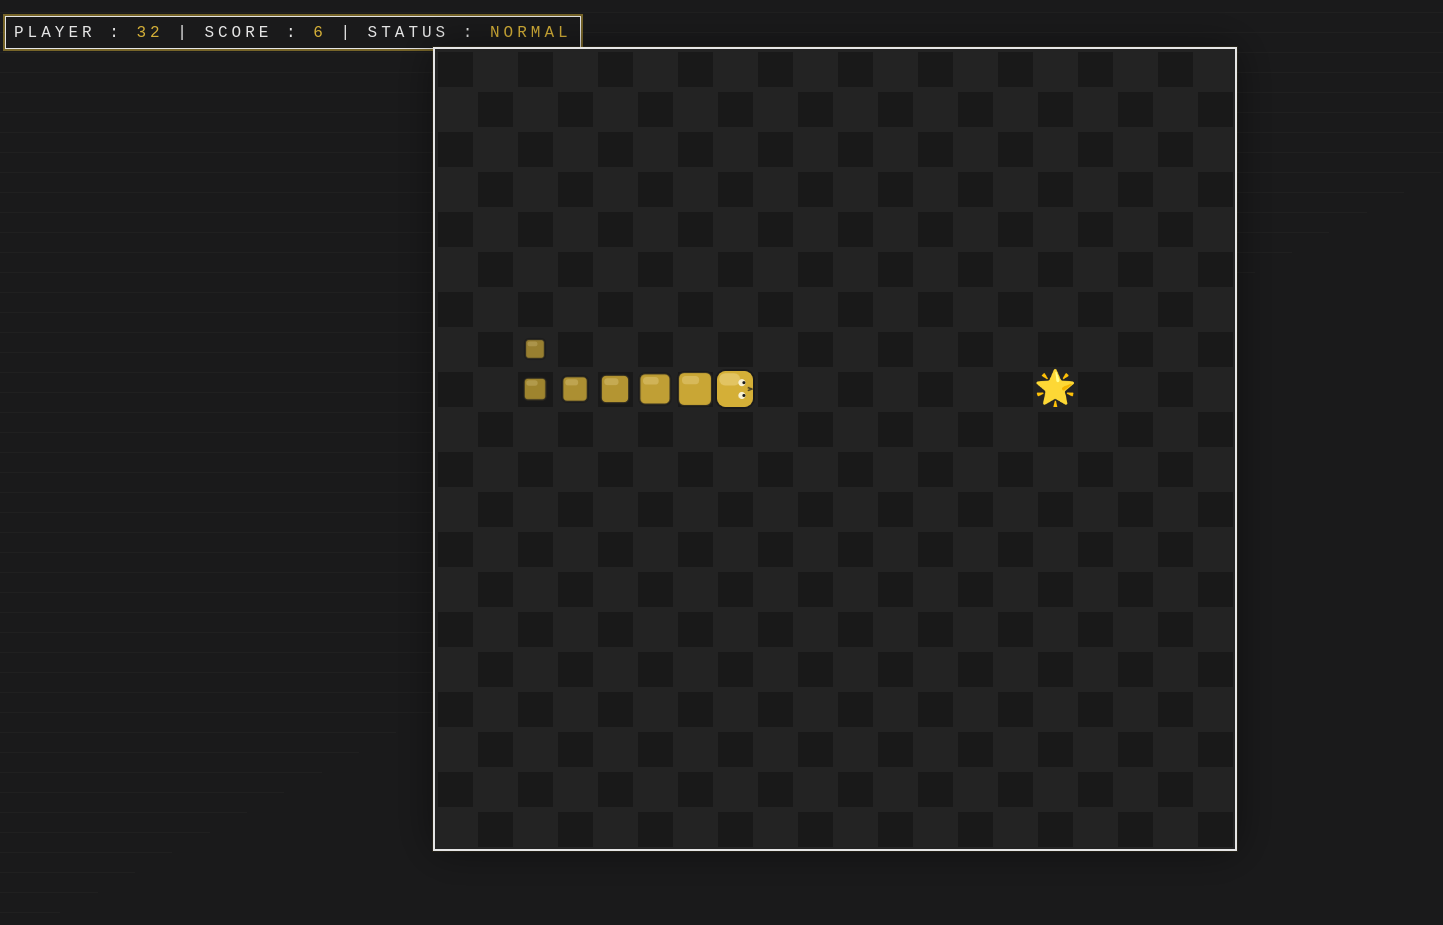
\includegraphics[width=0.8\textwidth]{Game.png}
    \caption{Game screen while running}
\end{figure}

\textbf{Immunity Mode}: During immunity, the snake wraps around border walls instead of dying, and pauses briefly on self-collision until the next directional input. A blue shield outline renders around the snake during this period and flickers in the final second as a warning. \textbf{When the immunity timer expires, a \texttt{removeExcess} function is automatically triggered. This feature evaluates the snake's body and removes all parts that are not directly connected to the snake head or are otherwise inconsistent with standard non-immune collision rules (such as disconnected segments left behind after wrapping through walls or passing through its own body).}

\textbf{Pause Menu \& Session High Score}: The player may press \texttt{Space} or \texttt{P} at any time to open a pause dialog offering Resume, Restart, and Home options. The game tracks the highest score achieved within the current browser session and displays it on the end screen after each game. All completed games are permanently stored via the backend server.

\sectionsep

%--- 4. Three-Layer Architecture ---%
\section{Three-Layer Architecture and Communication}

The project follows a three-layer structure: presentation, server, and administration.

\subsection{Frontend Layer}
The frontend consists of \texttt{index.html}, \texttt{style.css}, and \texttt{javascript.js}. HTML defines the page structure including inputs, configuration controls, the canvas, and dialogs. CSS provides dark-themed styling, gold-accented borders, backdrop blur panels, toggle switches, and responsive layout. JavaScript handles all game logic including movement, collision detection, food spawning, immunity mechanics, score tracking, and canvas rendering.

\subsection{Backend Layer}
The backend is implemented using Flask in \texttt{app.py}. It serves the HTML page and receives game results from JavaScript via an HTTP POST request. Upon receiving the data, it appends the record along with a server-side timestamp to the storage file.

\subsection{Administration Layer}
The administration layer is implemented in \texttt{admin.sh}. It reads the same history file and provides user search, recent scores, deletion, sorting, backup, and analytics through a menu-driven terminal interface.

\sectionsep

%--- 5. Communication ---%
\section{How Layers Communicate}

Communication occurs in the following sequence:
The player interacts with the browser interface. JavaScript computes the score and detects death conditions. When the game ends, JavaScript sends JSON data to Flask using an HTTP POST request. Flask receives the data and appends it to \texttt{history.txt}. The Bash admin script later reads the same file and performs management tasks. Therefore, \texttt{history.txt} acts as a shared storage medium connecting gameplay and administration.

\sectionsep

%--- 6. history.txt Format ---%
\section{Format Chosen for \texttt{history.txt} and Why}

Each line stores one completed game using comma-separated fields:
\begin{center}
\texttt{USERNAME,SCORE,DEATH\_CAUSE,SURVIVAL\_TIME,DD-MM-YYYY HH:MM:SS}
\end{center}

The fields represent username, score, cause of death (\texttt{WALL} or \texttt{SELF}), survival duration in seconds, and the timestamp logged by Flask. The comma separator was chosen because it integrates naturally with \texttt{awk}'s \texttt{-F','} field splitting used throughout the admin script. Since usernames do not contain commas and the timestamp format is fixed, the format remains unambiguous. One line per session keeps reading and processing simple and efficient.

\sectionsep

%--- 7. Administrative Features ---%
\section{Administrative Features}

The administration layer is implemented using a Bash script (\texttt{admin.sh}). It directly reads and processes the \texttt{history.txt} file without interacting with the backend, ensuring proper separation of concerns.

\subsection{User Selection and Filtering}

The script extracts unique usernames using:

\begin{lstlisting}
cut -d',' -f1 history.txt | sort | uniq
\end{lstlisting}

This allows operations to be performed on specific users.

\subsection{Viewing Recent Entries}

Recent game records are displayed using:

\begin{lstlisting}
tail -n 20 history.txt
\end{lstlisting}

\subsection{AWK-based Analytics}

The script computes mean score using:

\begin{lstlisting}
awk -F',' '{sum += $2; count++} END {print sum/count}'
\end{lstlisting}

Mean duration is computed similarly:

\begin{lstlisting}
awk -F',' '{dur += $4; count++} END {print dur/count}'
\end{lstlisting}

\subsection{Death Cause Analysis}

The script counts occurrences of different causes:

\begin{lstlisting}
if($3=="WALL") w++
else if($3=="SELF") s++
else if($3=="ENEMY") e++
\end{lstlisting}

These values are later used to calculate proportions.

\subsection{Timestamp Conversion Logic}

Timestamps are stored in the format:

\begin{verbatim}
DD-MM-YYYY HH:MM:SS
\end{verbatim}

To enable correct sorting, the date is rearranged:

\begin{lstlisting}
year = substr($5,7,4)
month = substr($5,4,2)
day = substr($5,1,2)
\end{lstlisting}

This converts it into:

\begin{verbatim}
YYYYMMDD
\end{verbatim}

\subsection{Sorting Records}

Sorting by score:

\begin{lstlisting}
sort -t',' -k2 -n history.txt
\end{lstlisting}

Sorting by timestamp (after conversion):

\begin{lstlisting}
awk -F',' '{print year month day "," $0}' | sort | cut -d',' -f2-
\end{lstlisting}

\subsection{Log Rotation}

Backup and trimming of logs is done using:

\begin{lstlisting}
tar -czf backup.tar.gz history.txt
tail -n 10 history.txt > temp && mv temp history.txt
\end{lstlisting}
\sectionsep

%--- 8. Hurdles ---%
\section{Hurdles Faced and Solutions}

\textbf{Frontend--backend integration}: Connecting JavaScript to Flask required careful use of JSON-formatted POST requests and proper Flask request handling via \texttt{request.get\_json()}.

\textbf{Persistent score storage}: Browser memory resets on refresh, so a text-based history file was used to preserve records permanently across sessions.

\textbf{Collision logic in immunity mode}: Wall and self-collisions behave differently during immunity. Separate conditional branches were created to handle normal death vs. wrap-around or pause behaviour.

\textbf{Variable-speed game loop}: Clearing and resetting \texttt{setInterval} each frame in variable-speed mode required careful management to avoid multiple overlapping intervals accumulating.

\textbf{Canvas rendering quality}: Achieving smooth snake visuals with rounded rectangles, per-segment opacity fade, and the shield outline required iterative tuning of the \texttt{roundRect} and \texttt{arc} calls in the drawing functions.

\sectionsep

%--- 9. 10 More Hours ---%
\section{What We Would Do Differently With 10 More Hours}

All core features are implemented and functional. Given additional time, improvements would focus on refinement and user experience rather.
Also given sufficient longer time new features could also be implemented.

\textbf{Theme and UI styling}: The most immediate improvement would be giving the player a choice of visual theme --- a light mode alongside the current dark mode, and perhaps two or three alternative game-board colour palettes. A theme selector on the instructions screen would let users personalise their experience before starting.

\textbf{Game screen templates}: Beyond colour, different board templates (e.g. a retro green-on-black terminal style, a neon palette, or a minimalist white grid) would add character.

\textbf{New Game Modes}: Adding new game modes such as having variable number of obstacles in the grid or multiple fruits or having teleportation portals added to the game under various modes

\textbf{Animations and polish}: Smoother food-spawn effects, a brief flash on score increment, and a more refined death screen transition would all improve perceived quality. Extra game modes would be the natural next step, such as a wall-mode with procedurally placed obstacles or a time-attack mode.

\sectionsep

%--- 10. Important Code Snippets ---%
\section{Important Code Snippets}

\noindent\begin{minipage}{\linewidth}
\textbf{Grid size and Canvas sizing in JavaScript:}
\begin{lstlisting}[]
const maxPossibleSize = Math.min(window.innerWidth * 0.85, window.innerHeight * 0.85);
tileCount = Math.floor(maxPossibleSize / gridSize);
canvasBlock.width = canvasBlock.height = tileCount * gridSize;
\end{lstlisting}
\end{minipage}
\vspace{1em}

\noindent\begin{minipage}{\linewidth}
\textbf{Variable speed update in Game Loop:}
\begin{lstlisting}[]
if (toggle.checked) {
    clearInterval(gameInterval);
    gameInterval = setInterval(runGame, (150 - 2 * Math.min(70, currentScore)));
}
\end{lstlisting}
\end{minipage}
\vspace{1em}

\noindent\begin{minipage}{\linewidth}
\textbf{Sending game result to Flask backend:}
\begin{lstlisting}[]
const gameData = {
    username: username.value,
    age: document.getElementById("age").value,
    score: currentScore,
    survival_time: duration,
    cause: cause
};
fetch('/save_score', {
    method: 'POST',
    headers: { 'Content-Type': 'application/json' },
    body: JSON.stringify(gameData)
});
\end{lstlisting}
\end{minipage}
\vspace{1em}

\noindent\begin{minipage}{\linewidth}
\textbf{Flask Route for Saving Score:}
\begin{lstlisting}[language=Python]
@app.route('/save_score', methods=['POST'])
def save_score():
    data = request.get_json()
    name     = data.get('username')
    score    = data.get('score')
    duration = data.get('survival_time')
    cause    = data.get('cause')
    with open(HISTORY, 'a') as f:
        f.write(f"{name},{score},{cause},{duration},"
                f"{datetime.datetime.now().strftime('%d-%m-%Y %H:%M:%S')}\n")
    return jsonify({"status": "success", "message": "Score recorded!"})
\end{lstlisting}
\end{minipage}
\vspace{1em}

\noindent\begin{minipage}{\linewidth}
\textbf{Global High Score extraction in Bash:}
\begin{lstlisting}[language=bash]
awk -F',' 'NF==5 {if($2>max) max=$2; usr=$1}
           END{print "Global Best:", usr, max}' "$FILE"
\end{lstlisting}
\end{minipage}
\vspace{1em}

\sectionsep

%--- 11. Conclusion ---%
\section{Conclusion}

Snake Stack is a complete mini full-stack project that combines web development, backend programming, and shell scripting. The project demonstrates the practical use of frontend technologies for interactive logic and rendering, Flask for server-side processing and routing, and Bash tools for robust data administration. It successfully extends the classic Snake concept with modern features such as dynamic grid configurations, flexible speed modes, immunity mechanics, and persistent analytical tracking.

\sectionsep

%--- 12. Bibliography ---%
\section{Bibliography}

\begin{enumerate}
    \item Flask Documentation: \url{https://flask.palletsprojects.com}
    \item Python Documentation: \url{https://docs.python.org/3}
    \item MDN Canvas API Reference: \url{https://developer.mozilla.org/en-US/docs/Web/API/Canvas_API}
    \item MDN Fetch API Reference: \url{https://developer.mozilla.org/en-US/docs/Web/API/Fetch_API}
    \item GNU Bash Manual: \url{https://www.gnu.org/software/bash/}
    \item GNU Awk Manual: \url{https://www.gnu.org/software/gawk/}
\end{enumerate}

\sectionsep

%--- 13. Makefile ---%
\section{Makefile}

Create a file named \texttt{Makefile} in the project root directory. Indentation \textbf{must} use a real tab character, not spaces.

\noindent\begin{minipage}{\linewidth}
\textbf{Makefile configuration:}
\begin{lstlisting}[language=make]
report:
	pdflatex report.tex
	pdflatex report.tex

clean:
	rm -f *.aux *.log *.out *.toc

open:
	xdg-open report.pdf
\end{lstlisting}
\end{minipage}
\vspace{1em}

\noindent\begin{minipage}{\linewidth}
\textbf{Compile using:}
\begin{lstlisting}[language=bash]
make report
\end{lstlisting}
\end{minipage}

\end{document}
